% TU Delft Beamer template
% Author: Maarten Abbink
% Delft University of Technology
% March 2014
% Version 2.0
% Based on original version 1.0 of Carl Schneider
\documentclass{beamer}
\usepackage[english]{babel}
\usepackage{calc}
\usepackage[absolute,overlay]{textpos}
\mode<presentation>{\usetheme{tud}}

\title[Physics based piano simulation]{Physics based piano simulation}
\subtitle{\normalsize{ICCP 2015}}
\institute[TU Delft]{Delft University of Technology}
\author{Selwyn, Kenneth, Dani\"{e}l}
\date{\today}

% Insert frame before each subsection (requires 2 latex runs)
\AtBeginSubsection[] {
	\begin{frame}<beamer>\frametitle{\titleSubsec}
		\tableofcontents[currentsection,currentsubsection]  % Generation of the Table of Contents
	\end{frame}
}
% Define the title of each inserted pre-subsction frame
\newcommand*\titleSubsec{Next Subsection}
% Define the title of the "Table of Contents" frame
\newcommand*\titleTOC{Outline}

% define a symbol which can be removed if you don't need it
\newcommand{\field}[1]{\mathbb{#1}}
\newcommand{\Zset}{\field{Z}}

\begin{document}

{
% remove the next line if you don't want a background image
\usebackgroundtemplate{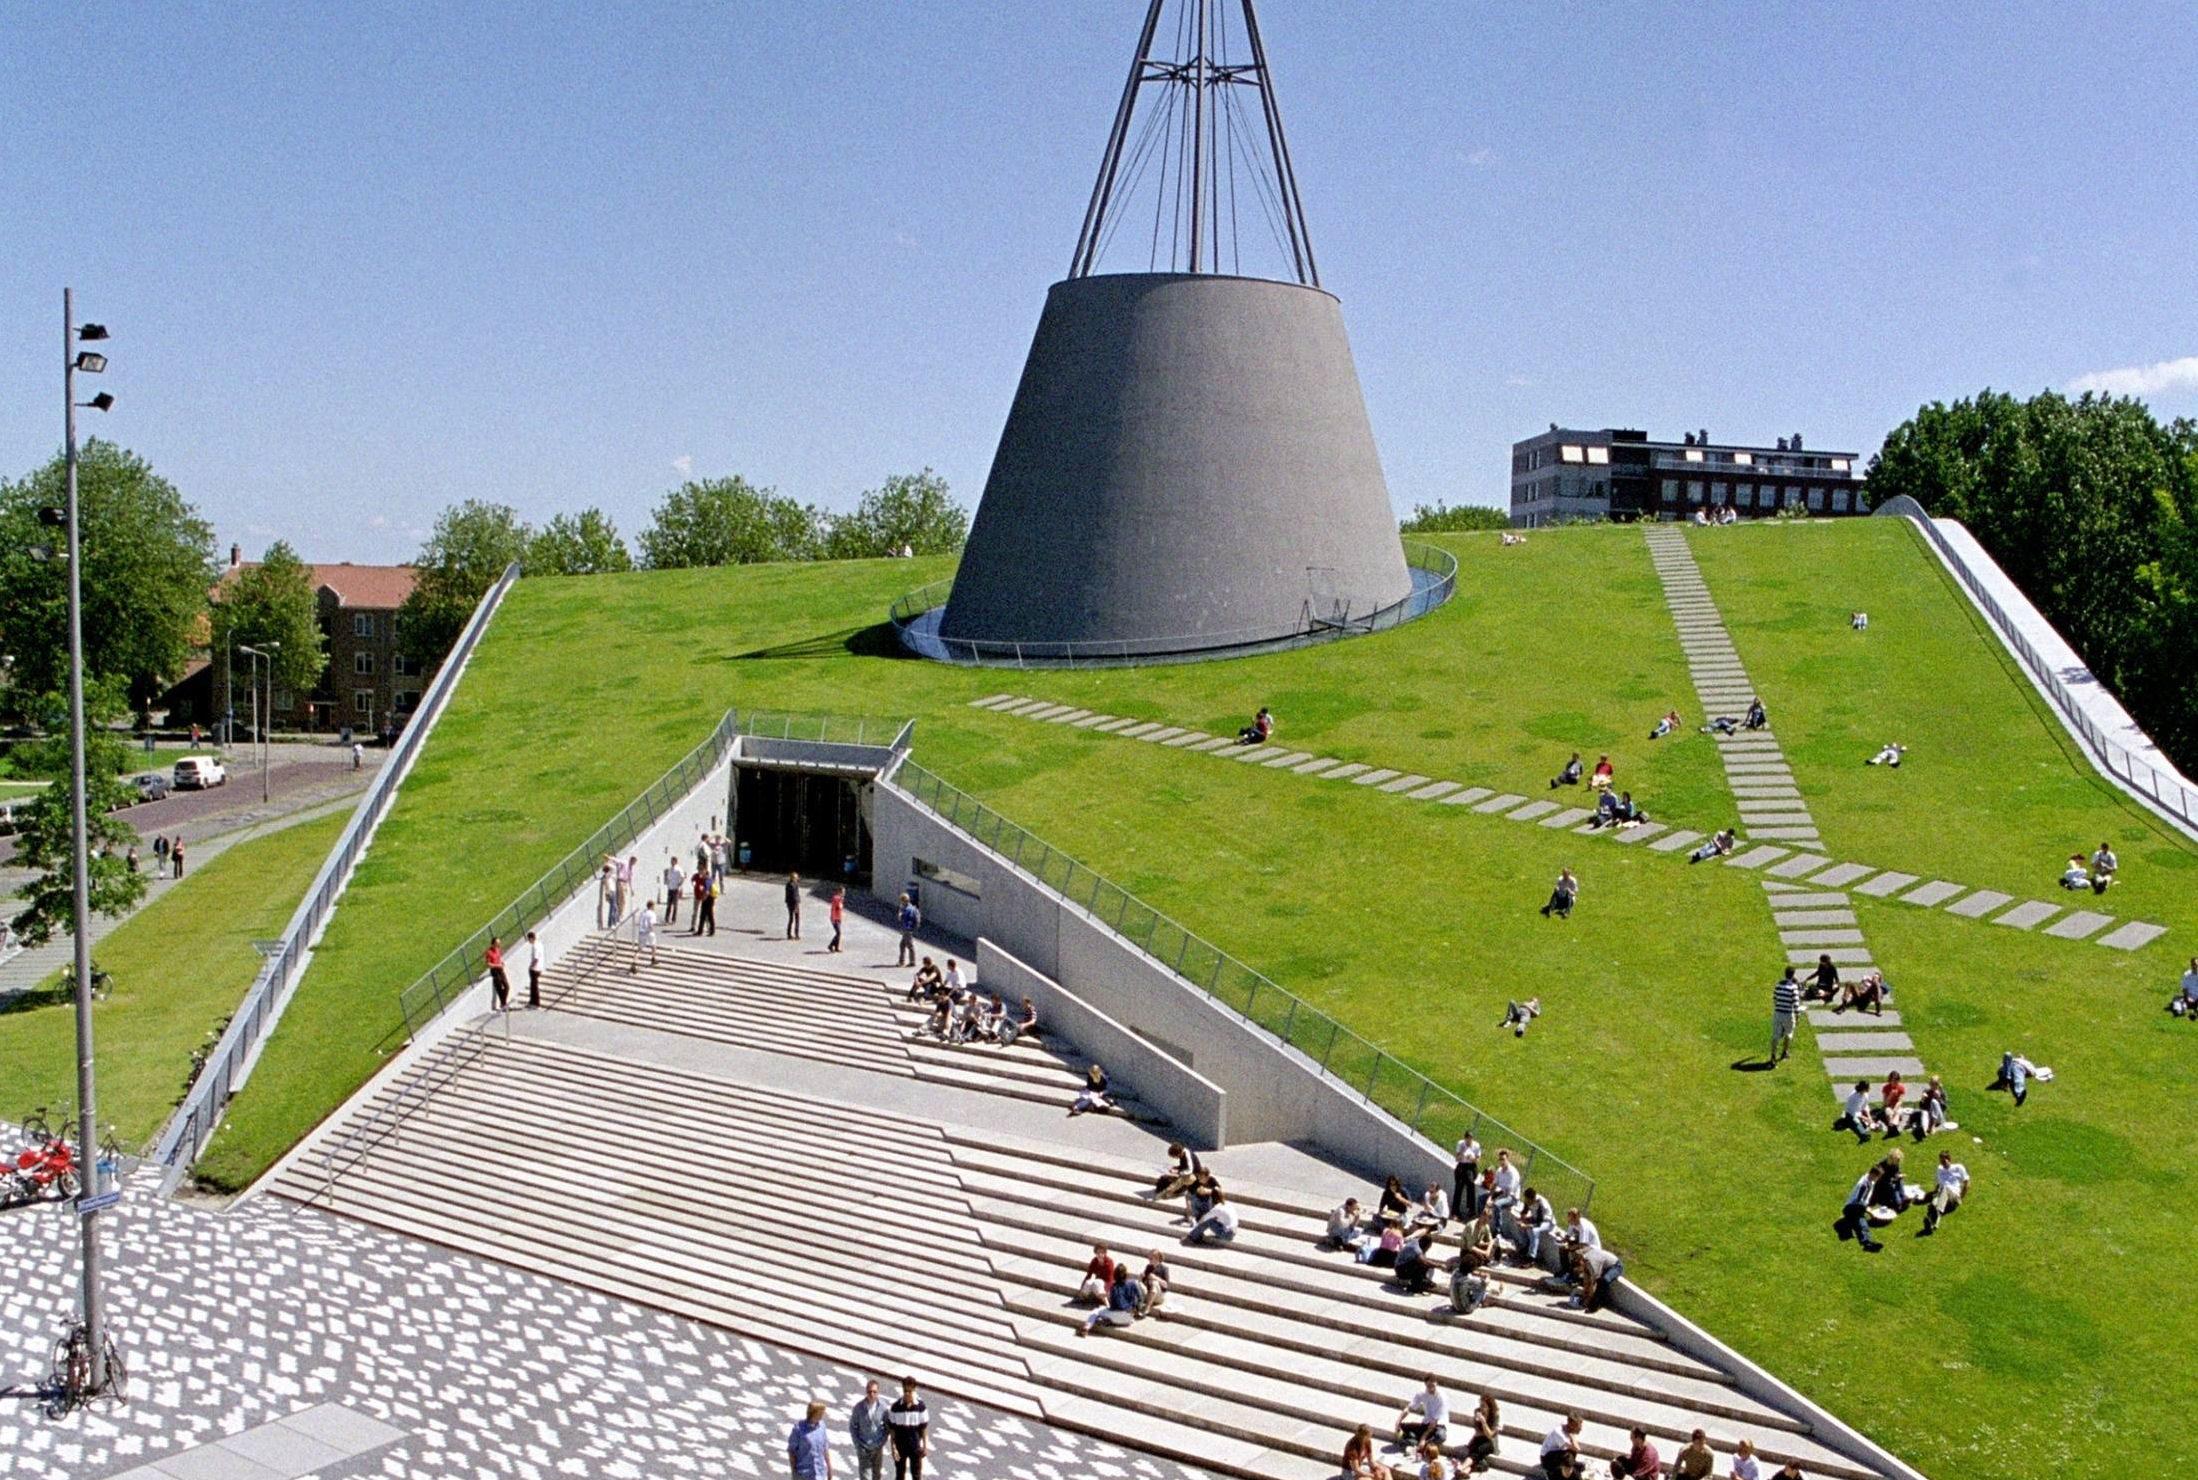
\includegraphics[width=\paperwidth,height=\paperheight]{images/background-titlepage.jpg}}%
\setbeamertemplate{footline}{\usebeamertemplate*{minimal footline}}
\frame{\titlepage}
}

{\setbeamertemplate{footline}{\usebeamertemplate*{minimal footline}}
%\begin{frame}\frametitle{\titleTOC}
%	\tableofcontents
%\end{frame}
}
\begin{frame}\frametitle{Simplified piano string interaction}
	
		\begin{minipage}{1\textwidth}
			% insert picture (pdf file)
			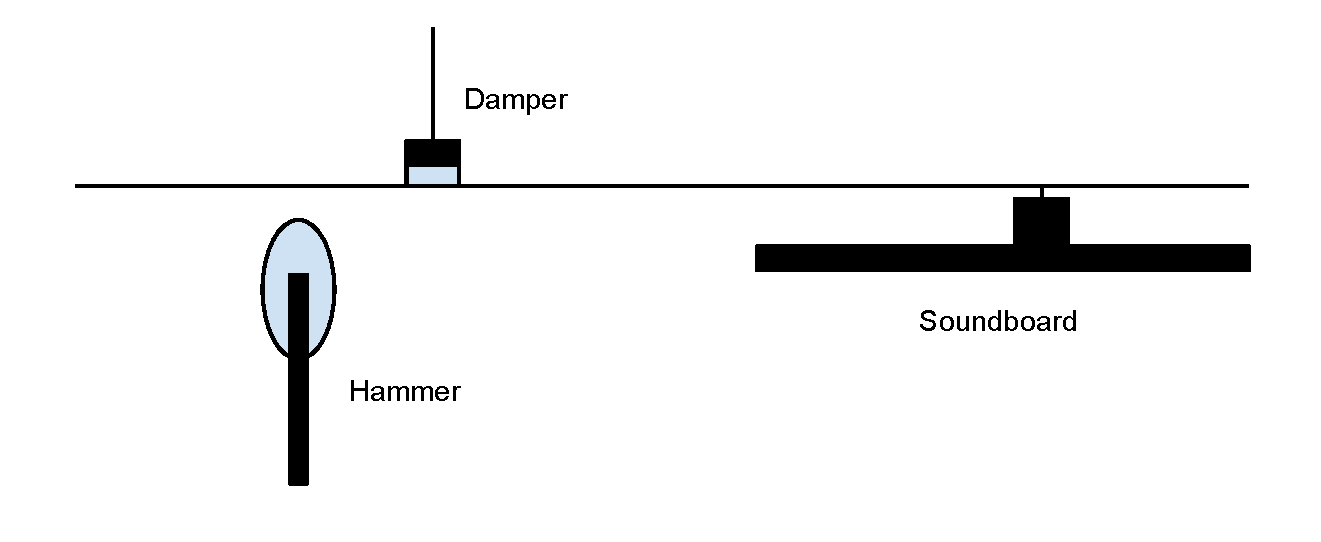
\includegraphics[width=\textwidth]{images/string.pdf}
		\end{minipage}
\end{frame}

\begin{frame}\frametitle{The wave equation}
	\begin{gather*}
	\frac{\partial^2 y}{\partial t^2} = c^2\frac{\partial^2 y}{\partial x^2}-\kappa^2\frac{\partial^4y}{\partial x^4}-2b_1\frac{\partial y}{\partial t} + 2b_2 \frac{\partial^3y}{\partial x^2\partial t}\\
\end{gather*}
\end{frame}

\begin{frame}\frametitle{Finite difference wave equation}
	\begin{gather*}
	\frac{\partial^2 y}{\partial t^2} = c^2\frac{\partial^2 y}{\partial x^2}-\kappa^2\frac{\partial^4y}{\partial x^4}-2b_1\frac{\partial y}{\partial t} + 2b_2 \frac{\partial^3y}{\partial x^2\partial t}\\
y_n^{t+1} = a_1\left(y_{n+2}^t+y_{n-2}^t\right)+a_2\left(y_{n+1}^t+y_{n-1}^t\right)+a_3y_n^t\\
+a_4y_n^{t-1}+a_5\left(y_{n+1}^{t-1}+y_{n-1}^{t-1}\right)\\
a_i depends on string stiffness, Young's modulus, tension, length, cross-section...
\end{gather*}
\end{frame}


\begin{frame}\frametitle{Hammer strike}
Hammer-string interaction:\\

\begin{gather*}
L = T - V = \sum_i \frac{1}{2}M_H\dot{x_i}^2+\sum\frac{1}{2}\rho \Delta x \dot{\eta}^2-(\eta_n-x_n)^{b+1}\frac{K}{b-1}\\+V_{string}\left(\eta_1,\eta_2,\cdots, \eta_n\right)\\
\frac{\partial}{\partial t}\frac{\partial L}{\partial \dot{x}_n} = M_H\ddot{x} = \frac{\partial L}{\partial x} = \sum_n-\left(\eta_n-x_ n\right)^bK\\
\frac{\partial}{\partial t}\frac{\partial L}{\partial \dot{\eta}_n} = \rho \delta x \ddot{\eta}_n = \frac{\partial L}{\partial \dot{\eta}_n} = k(\eta_n-x_n)^b - \frac{\partial V_{string}\left(\eta_1,\eta_2,\cdots, \eta_n\right)}{\partial \eta_n}
\end{gather*}
\end{frame}

\begin{frame}\frametitle{Hammer strike}
\begin{gather*}
\ddot{x}_n = -\frac{k}{M_H}\sum_n (\eta_n-x_m)^bH(\eta_n-x_m)\ddot{\eta}_n = \frac{k}{\rho\Delta x}\left(\eta_n-x_n\right)^b+\frac{1}{\rho\Delta x}F_n\\
x_n(t+\Delta t) = x_n(t) + v_n(t)\Delta t + \frac{k}{2M_H}\left(\eta_n(t)-x_n(t)\right)^bH(\eta_n,x_n)\\
\dot{x}_n(t+\delta t) = \dot{x}_n(t) + \delta t \frac{\left(\eta_n-x_n\right)^b+\left(\eta_n-x_n(t)\right)^b}{2}\\
\eta_n(t+\Delta t) = \eta_n(t) + v_n(t)\Delta t + \frac{k\left(\eta_n-x_n(t)\right)^b}{2\rho \Delta x}\left(\Delta t\right)^2
\end{gather*}
\end{frame}


\begin{frame}\frametitle{Hammer strike}
Hammer release from the string, important for 'plucking' or 'striking' the string.
\end{frame}


\begin{frame}\frametitle{Frequency spectrum}
\begin{minipage}{1\textwidth}
		% insert picture (pdf file)
		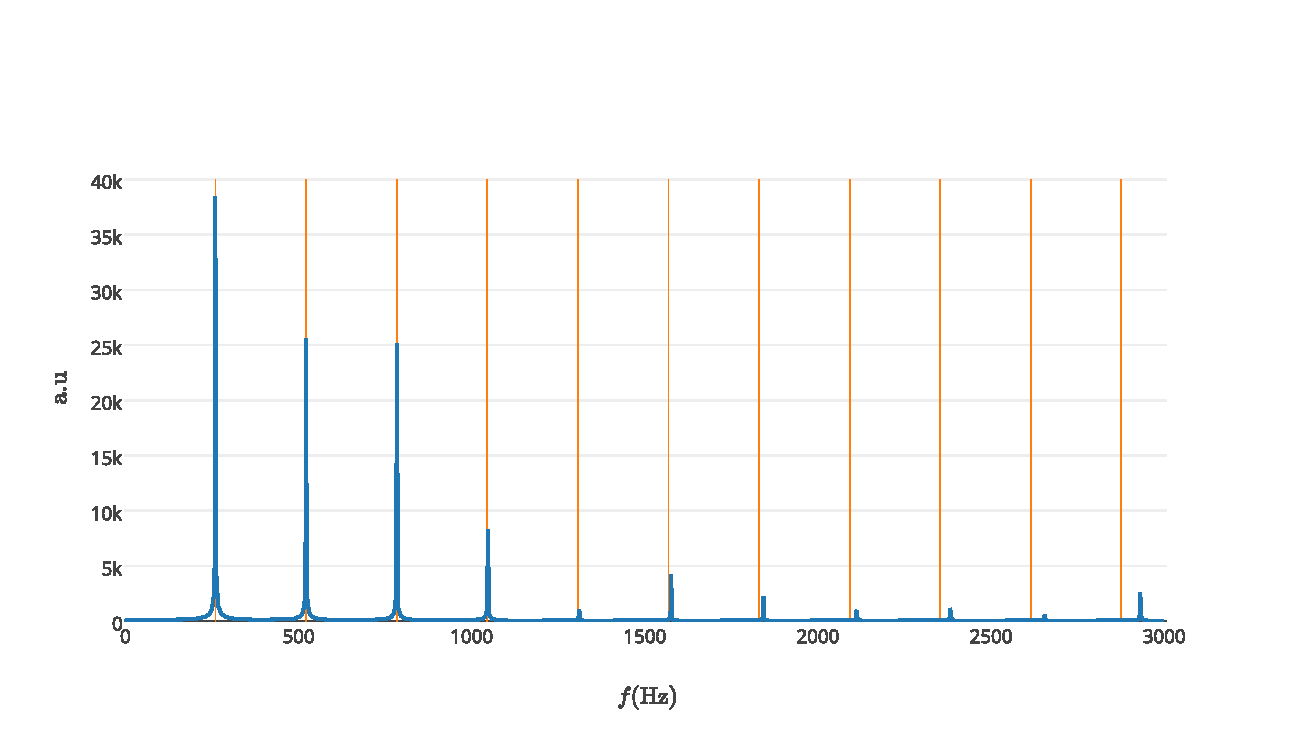
\includegraphics[width=\textwidth]{images/freq.pdf}
	\end{minipage}
\end{frame}

\begin{frame}\frametitle{Damper simulation}
Cutoff sounds unnatural
\end{frame}

\begin{frame}\frametitle{Damper simulation}
Cutoff sounds unnatural $\rightarrow$ add damper suppression
\end{frame}

\begin{frame}\frametitle{Damper simulation}
Cutoff sounds unnatural$\rightarrow$ add damper suppression\\
Suddenly increase stiffness
\end{frame}

\begin{frame}\frametitle{Damper simulation}

    \begin{minipage}{0.47\textwidth}
		% insert picture (pdf file)
		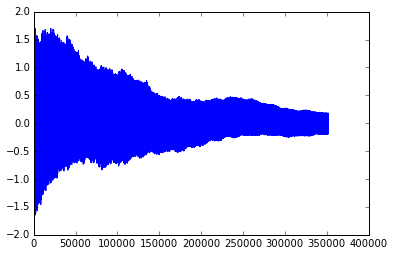
\includegraphics[width=\textwidth]{images/normal.png}
	\end{minipage}
    \begin{minipage}{0.47\textwidth}
		% insert picture (pdf file)
		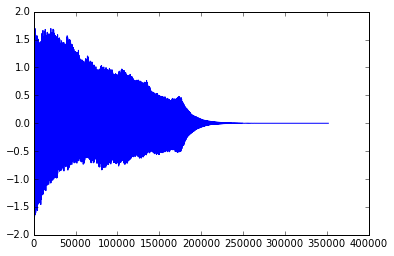
\includegraphics[width=\textwidth]{images/damped.png}
	\end{minipage}
\end{frame}



\begin{frame}\frametitle{Examples}
Time for some 'music'!
\end{frame}

\begin{frame}\frametitle{Considerations}
\begin{itemize}
\item Add more notes
\end{itemize}
\end{frame}


\begin{frame}\frametitle{Considerations}
\begin{itemize}
\item Add more notes
\item Real-time playback
\end{itemize}
\end{frame}

\begin{frame}\frametitle{Considerations}
\begin{itemize}
\item Add more notes
\item Real-time playback
\item Simulate three strings of same pitch with slightly different parameters
\end{itemize}
\end{frame}


\begin{frame}\frametitle{Last Page}
		\centering{Thank you!}
\end{frame}

\end{document}
